\documentclass[12pt]{article}
\usepackage[utf8]{inputenc}
\usepackage[ruled, vlined]{algorithm2e}
\usepackage{amsmath}
\usepackage{amssymb}
\usepackage{biblatex}
\usepackage{booktabs}
\usepackage{caption}
\usepackage{cancel}
\usepackage{color}
\usepackage[export]{adjustbox}
\usepackage{graphicx}
\usepackage{hyperref}
\hypersetup{colorlinks=true, linkcolor=red,  filecolor=cyan, urlcolor=blue,}
\usepackage{float}
\usepackage[margin=1in]{geometry}
%\usepackage{nopageno}
\usepackage{nomencl}
\usepackage{titlesec}
\graphicspath{ {Images/} }
\renewcommand{\baselinestretch}{1.2}
\setlength\parindent{0pt}
\setlength{\parskip}{\baselineskip}
\newcommand\tab[1][1cm]{\hspace*{#1}}
\usepackage{setspace}
\usepackage{listings}
\numberwithin{equation}{section}
\usepackage{xcolor}


%\makenomenclature
%\addcontentsline{}{}{}
%\usepackage[linktoc=all]{hyperref}
%\usepackage[linktocpage=true]{hyperref}

\begin{document}
% ------------------------------- Title Page --------------------------- %
\begin{titlepage}
% ------------------------------------------------------------------------- %
\newcommand{\HRule}{\rule{\linewidth}{0.5mm}}
\center
\textsc{\LARGE Technion - Israel Institute of Technology}\\[0.6cm]
{\large \textbf{Machine Learning in Healthcare (097248)}}\\[0.6cm]
{\large \textbf{Wisconsin Breast Cancer Dataset}}\\[1.25cm]

% ------------------------------------------------------------------------- % 
\begin{figure}[H]
\centering
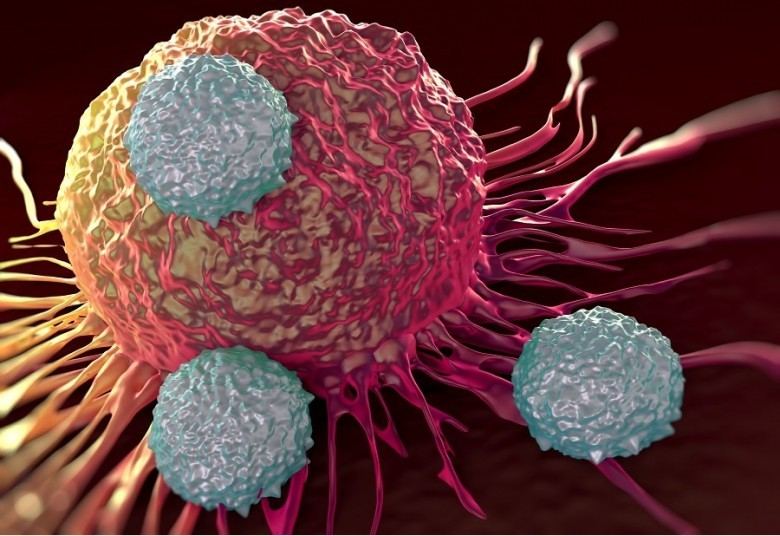
\includegraphics[scale=0.451]{Intro_2.png}
\end{figure} 
% ------------------------------------------------------------------------- % 
\begin{figure}[H]
\centering
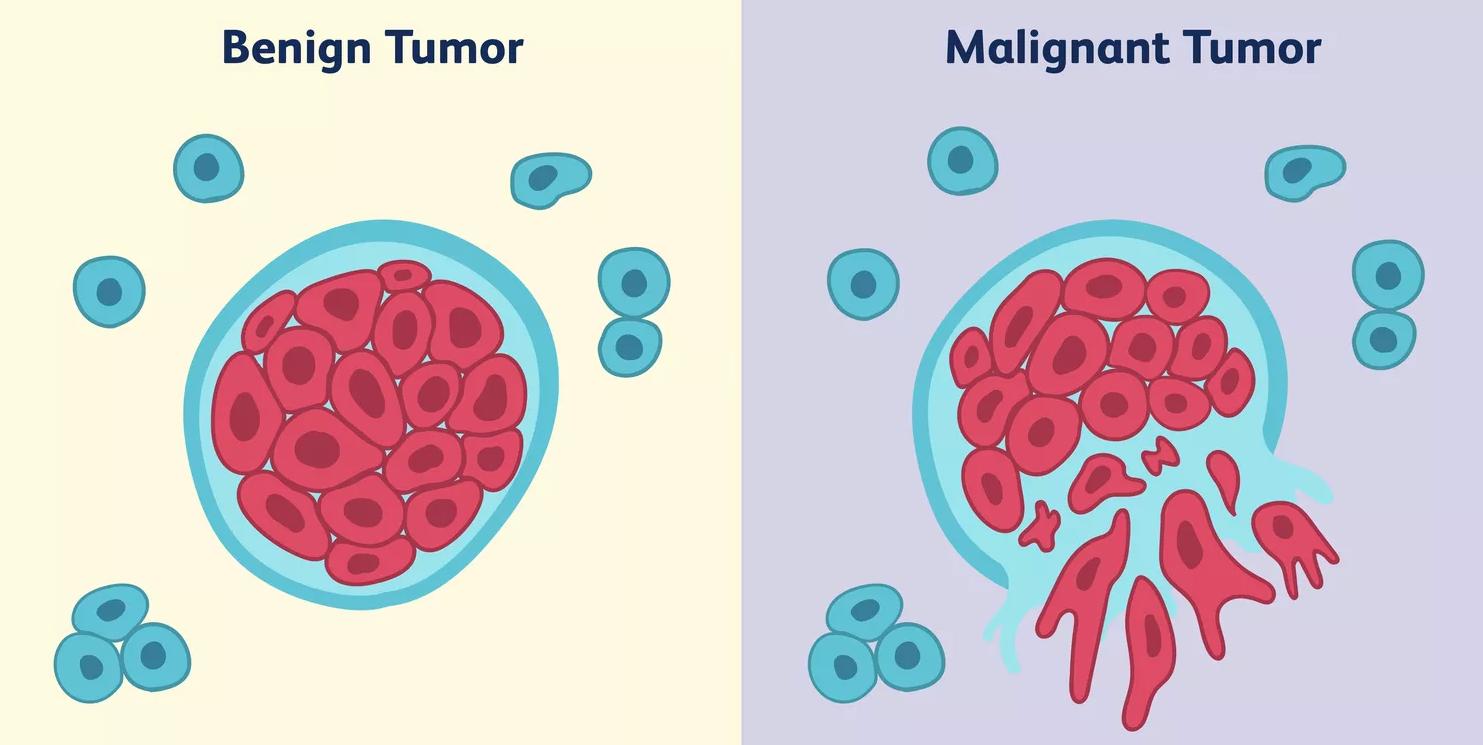
\includegraphics[scale=0.2375]{Intro_3.png}
\end{figure} 
% ------------------------------------------------------------------------- % 
\HRule \\[0.2cm]
\textbf{Daniel Engelsman @ {\today}}\\[0.1cm]
\HRule \\
% ------------------------------------------------------------------------- %
\end{titlepage}

\begin{flushleft} 
\pagenumbering{gobble} % exclude page number of TOC
\begingroup
\hypersetup{linkcolor=black}
\renewcommand{\baselinestretch}{0.85}\normalsize
\tableofcontents 
\renewcommand{\baselinestretch}{1.0}\normalsize
\endgroup 				% reduce items spacing
\newpage

\pagenumbering{arabic} % activate page number
% --------------------------------------------------------------------------------------------------- %
\hypersetup{linkcolor=red}

%\subsection*{Abstract}  \addcontentsline{toc}{subsection}{Abstract}


\section{Description of the Problem}

\textbf{Breast cancer} is a form of cancer that develops from breast tissue. The most common risk factors include : being female, obesity, a lack of physical exercise, alcoholism, an early age at first menstruation, having children late in life or not at all, older age and a family history of breast cancer [\ref{Intro_1}]. Typically it presents as a lump that feels different from the rest of the breast tissue, often self detected by the person's fingertips.

Cancer grows by simple cell division. It begins as one malignant cell, which then divides and becomes two bad cells and so forth. Each division takes about two months [\ref{Intro_2}], and detection by hand cannot be felt before the 30th division, hence pre-existence of 2-3 years. 

The earliest breast detection are obtained by a mammogram : an X-rays screening method that can offer an approximate likelihood whether a lump is cancerous. When examinations are inconclusive, a healthcare provider can remove a sample of the lump fluid / biopsy, and then examine it deeper under a microscopic analysis (\href{https://en.wikipedia.org/wiki/Fine-needle_aspiration}{FNA}) : \vspace{0.6cm}

\begin{figure}[H]
\centering
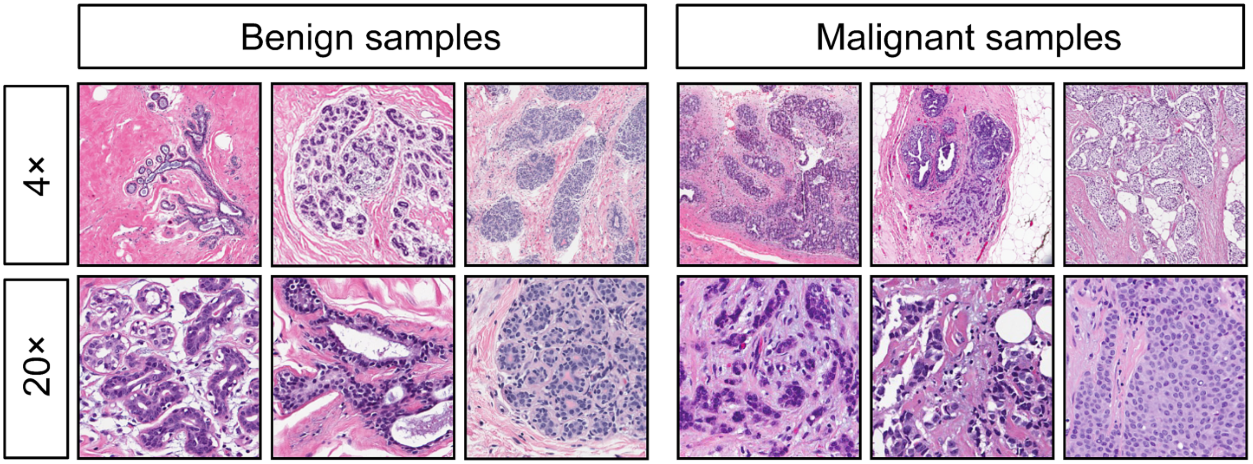
\includegraphics[scale=0.375]{Benign_Malignant.png}
\end{figure} 
Visual differences between benign (non-cancerous) and malignant (cancerous) cells can be very elusive at early detection stages. Researchers rely on typical dissimilarities of each cell's characteristics (perimeter, area, texture etc.) to diagnose its status (\href{https://www.radiologyinfo.org/en/info.cfm?pg=breast-cancer}{ACR}).

For this reason, the pre-diagnosis allows a narrow window of opportunity that can be lifesaving, before the cancer spreads to secondary sites (Metastasis). Thus, analysis is extremely important and should be handled by experts only.

\newpage

\subsection{Why AI ?}

As seen from articles along the semester, clinicians, regardless their years of experience and expertise, eventually make mistakes. These wrong indications accumulate over time, resulting in high rates of false positives and false negatives (FPR / FNR) [\ref{Intro_3}]. 

Contrarily, AI systems have proven to outperform radiologists when it comes to interpreting breast cancer mammograms, resulting in higher area under the operating characteristic curve (\textbf{AUC-ROC}) [\ref{Intro_4}]. Exploiting the vast amounts of labeled data in the electronic health records (EHR) makes the AI frameworks helpful in fight against cancer [\ref{Intro_5}].

\section{Background and Related Work}
The Wisconsin Breast Cancer Dataset (\href{https://archive.ics.uci.edu/ml/datasets/Breast+Cancer+Wisconsin+(Diagnostic)}{WBCD}) was first released on 1992 by Wisconsin university, and since became a milestone in the AI progress. However, early publications utilized mainly classic machine learning methods due to primitive computational platforms. 

Bennett et al. (1992) [\ref{BG_1}] proposed a minimization scheme which reduces the average sum of misclassified points belonging to two disjoint points sets in $\mathbb{R}^{n}$ space. Disjoint of the two convex subsets leads to a complete separation plane between them. 

Street et al. (1993) [\ref{BG_2}] used ten-fold cross-validation on a single separating plane utilizing only three most important features. Mangasarian (1995) [\ref{BG_3}] showed how linear programming (LP) techniques are capable of minimizing a penalty over a misclassified points, thus converging to almost perfect classification.

Y-J Lee (2000) [\ref{BG_4}] utilized a linear support vector machine (SVM) to extract 6 features from a total 30. Then, using Gaussian kernel non-linear SVM, the reduced dataset underwent division into three prognostic groups, ending up with a high level of accuracy.

The progress in artificial neural networks (ANN) in the beginning of the 2000s opened the door for many novel approaches. Pantazi (2002) [\ref{BG_5}] showed how Kohonen model of self-organizing maps can be utilized for cluster analysis on the WBCD. Revett [\ref{BG_6}] et al. (2005) presented a medical decision system based on a probabilistic NN to perform dimensionality reduction to eliminate redundant attributes from the dataset. 

Huang et al. (2007) [\ref{BG_7}] were first to achieved an outstanding classification accuracy of $98.14 \%$ by hybridizing a fuzzy-artificial immune system with k-nearest neighbor algorithm. 

Belciug (2010) [\ref{BG_8}] assessed the effectiveness of three different clustering algorithms with respect to the WBCD, by comparing the performance of a classical k-means algorithm with a much more sophisticated methods : SOM-Kohonen network and a cluster network. \\[0.6cm]

\textbf{The "big bang" of the deep learning (DL)}

%\subsubsection*{The "big bang" of the deep learning (DL)}
Since 2012, the ImageNet project is responsible for many technological breakthroughs. Nowadays, a simple deep learning (DL) model can easily obtain a precise classification. These models manage to automatically redundant tough procedures e.g dimensionality reduction, decimation and feature extraction, outputting eventually impressive results.

Karthik et al. (2016) [\ref{BG_9}] showed how Computer-Aided Diagnosis (CAD) can employ DNN as classifier model and recursive feature elimination (RFE) for feature selection. After optimizing the train-test split the model reached $98.62 \%$ accuracy. 

Abdel-Zaher et al. (2018) [\ref{BG_10}] presented a CAD detection scheme using deep belief network unsupervised path (DBN-NN), achieving $99.68 \%$ accuracy rate and $100 \%$ sensitivity.

%To conclude, technology and research advancements kept raising the accuracy bar, resulting in almost perfect classification of the WBCD samples. 

\subsection{Intention Statement}
In this project I aim to explore the data thoroughly, in search of hidden patterns using \underline{non deep learning} classification tools. The findings will be analyzed in context of the problem's clinical aspects using interactive data visualizations. This way I hope to establish a robust understanding of machine learning in context of \underline{healthcare}.

\subsection{The workflow}

\begin{figure}[H]
\centering
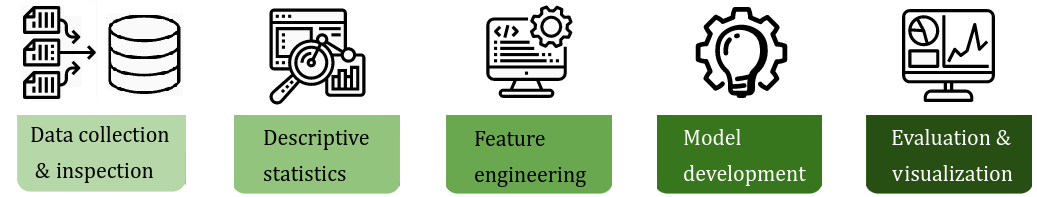
\includegraphics[scale=0.45]{pipeline.png}
\end{figure} 

\newpage

\section{Description of the Data}
The raw dataset (including indices and \textbf{id}) after applying random shuffling [ \href{https://archive.ics.uci.edu/ml/machine-learning-databases/breast-cancer-wisconsin/wdbc.data}{\underline{ $\downarrow$ }} ] : \\[0.2cm]
\begin{figure}[H]
\centering
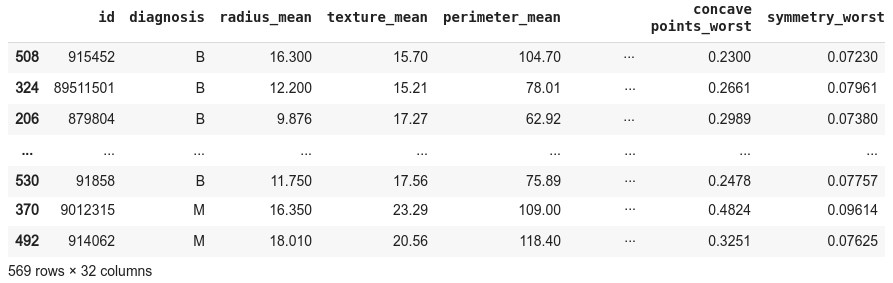
\includegraphics[scale=0.55]{data_table.png}
\end{figure}
${\text{Number of samples }} : n = 569  \hspace{3.1cm} {\text{Full dataset}} : \ D = \{ X, Y \} = \{ x_i, y_i \}_{i=1}^{n}$ \\[0.1cm]

$ \text{Input space : }  \dim(X) = ( \underset{\text{case :}}{n \times 10}) \times \underset{\text{\textbf{a, b, c}}}{3} \tab \text{Output space : }\dim(Y) = n $  \\ \vspace{3mm}

$\underline{\text{Dependent variable / Target}} \ \big( \hspace{2mm} y_i = \{B, \, M  \} \hspace{2mm} \big)$ \\ \vspace{2mm}
\tab  \textbf{Diagnosis} - Binary indication whether a sample is Benign $(0)$ or Malignant $(1)$.

Feature space $X$ consists of three different analysis cases (\underline{same} features) : \\[2mm]
\textbf{a} $:=$ Mean $(\mu) =  X_{[:, \, 1:10]} \hspace{0.1cm}$ \hspace{2mm}
\textbf{b} $:=$ SE $(\frac{\sigma}{\sqrt{n}})  = X_{[:, \, 11:20]}$ \hspace{1.5mm}
\textbf{c} $:=$ Worst (3 max-values) $ = X_{[:, \, 21:30]}$ \\[0.4cm]

For example, let us examine the $i$-th sample from the mean case (\textbf{a}) : \\[2mm]
$\underline{\text{Independent variable / Feature}} \,\ \big( \hspace{2mm} x_i \in \mathbb{R}^{10} \hspace{2mm} \big)$  \\ \vspace{2mm}
\tab \textbf{Radius} - mean of distances from center to points on the perimeter. \\
\tab \textbf{Texture} - standard deviation of gray-scale value. \\
\tab \textbf{Perimeter} - $P = \sum_{i=1}^n l_i \hspace{39.25mm}$ (Given  $n$  vertices) \\
\tab \textbf{Area} - $\hspace{7mm} A = \frac{1}{2} \big( \sum_j w_j z_{j+1} - z_{j} w_{j+1} \big) \hspace{1.3cm}$ (Given  $n$  vertices on WZ plane) \\
\tab \textbf{Smoothness} - Local variation in radius lengths. \\
\tab \textbf{Compactness} - ($P^2$ / $A$ - 1.0) \\
\tab \textbf{Concavity} - Severity of concave portions of the contour. \\
\tab \textbf{Concave points} - Number of concave portions of the contour. \\
\tab \textbf{Symmetry} - Relative difference of two half-planes. \\
\tab \textbf{Fractal dimension} - ("coastline approximation" - 1)\\[2mm]
To sum up, the dataset is composed such that : $X = [X^{(a)}_{\text{Mean}}, \, X^{(b)}_{\text{SE}}, \, X^{(c)}_{\text{Worst}}] \in \mathbb{R}^{(n \times 10) \times 3}$

\subsection{Data composition}
\begin{figure}[H]
\centering
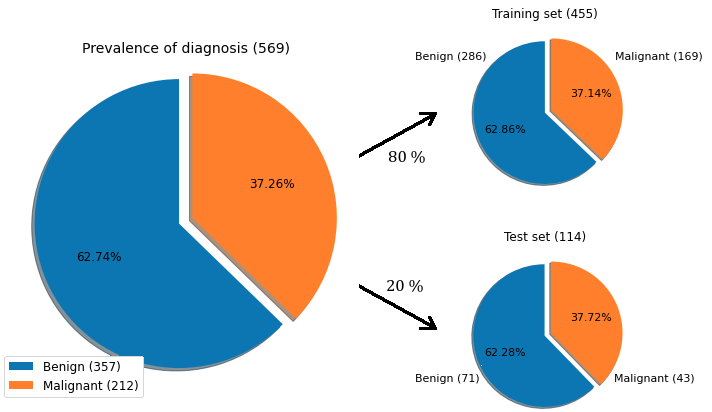
\includegraphics[width=0.82\linewidth, center]{train_split.png}
\end{figure}
Although division is not perfectly balanced, it is sufficiently good. The first manipulation will help us gaining some intuition by comparing the mean value of every feature :
\begin{figure}[H]
\centering
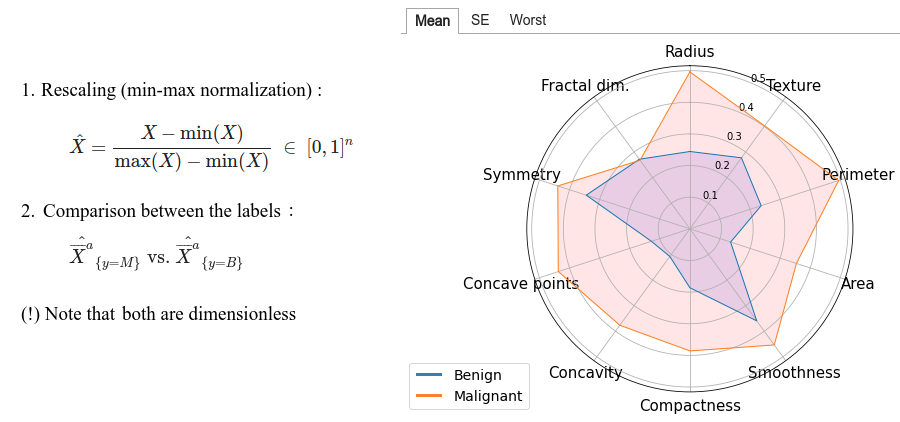
\includegraphics[width=1.045\linewidth, center]{comparison.png}
\end{figure}
This presentation is useful as it compares the classes by measure of similarity  $d(B,M)$. \\
\textbf{\underline{Note} :} Interactive switching between the tabs (cases) is available via the \textit{Colab}\\ \hspace{13.5mm} version. Anyway, for the sake of analysis, I will refer to all of the cases.

\textbf{True for all} : Almost all cases exhibited higher feature values in the malignant class. However, Fractal dimension seemed to be equal for both - $d(B,M) \approx 0$.


\textbf{Mean case (a)} : The most important comparison (above) as it manages to capture most of the feature dissimilarities between $\ (B/M) \ $ : \\[0.1cm]
$\hspace{1cm} \bullet$ Proximity - \hspace{3.3mm} $d(B,M) \leq 0.1$ : Symmetry, Smoothness \\[0.1cm]

$\hspace{1cm} \bullet$ Dissimilarity - $d(B,M) > 0.1$ : The remained features 

\textbf{Standatd Error case (b)} : The differences in the SE comparison are significantly smaller, implying that the SE group distributes \underline{uniformly}, and is useless for any inference.

\textbf{Worst case (c)} : Resembles \textbf{(a)} case, where the $M$ features are much greater than $B$.

%To sum up, the above graph provides some intuition on the $B / M$ differences. 

\subsection{Statistical analysis}
 
\begin{figure}[H] 
\centering
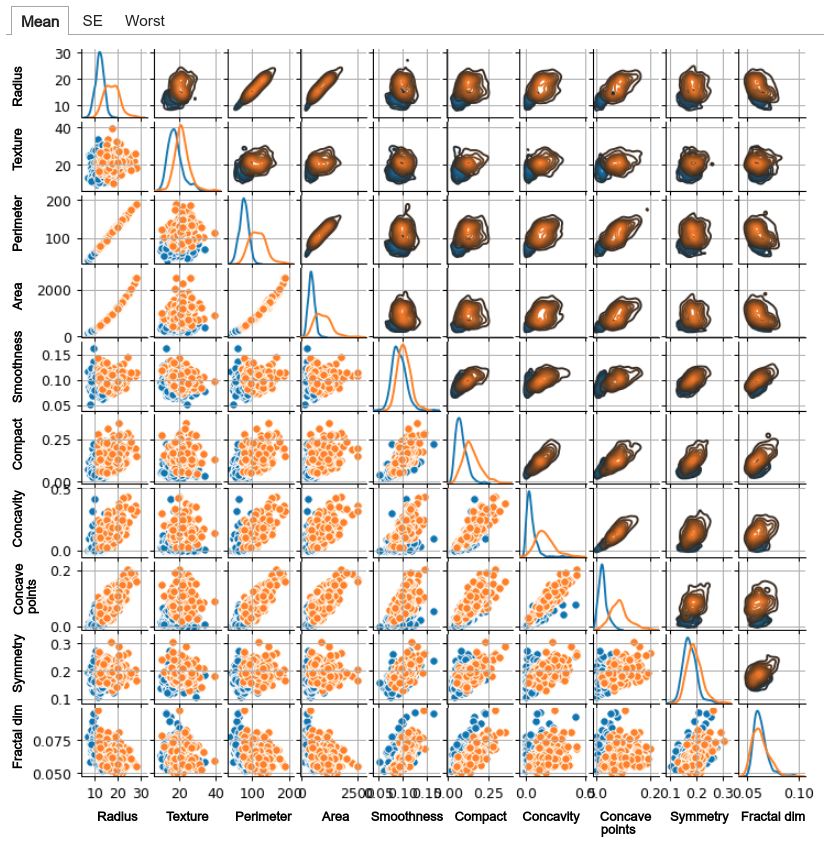
\includegraphics[width=0.773\linewidth, center]{Statistics.png}
\end{figure}

The above table maps each independent variable onto a row and column in a grid of multiple axes in order to explore bivariate relationships between every feature pair. The \textbf{lower} triangular presents a raw scatter plot of the joint probability distribution $P_{XY}(x, y)$. The \textbf{upper} triangular presents the same, using KDE smoothed contour lines. \\ The \textbf{diagonal} exhibits the marginal distribution of both variables - $P_{X}(x) \, , \, P_{Y}(y)$ .

This analysis shows not only the $(B/M)$ differences but also the way each feature distributes. Smoothness and Fractal dimension distributes similarly, hence helpless in the classification attempt. In contrast, Concavity and Radius show significant difference.

In order to better understand which features contribute most, an efficient method can be calculating the Pearson correlation coefficients to obtain a correlation matrix. Thereby, the strength of linear relationships are obtained in two aspects (\hyperlink{corr_mat}{Appendix A}) : \\[3mm]
\tab $(i) \hspace{1mm} $ \textbf{feature} vs. \textbf{feature} - Every pair of two independent variables. \\
\tab  $(ii)$ \textbf{feature} vs. \textbf{target} \ - Every pair of feature-target (bottom rectangle).

\begin{figure}[H]
\centering
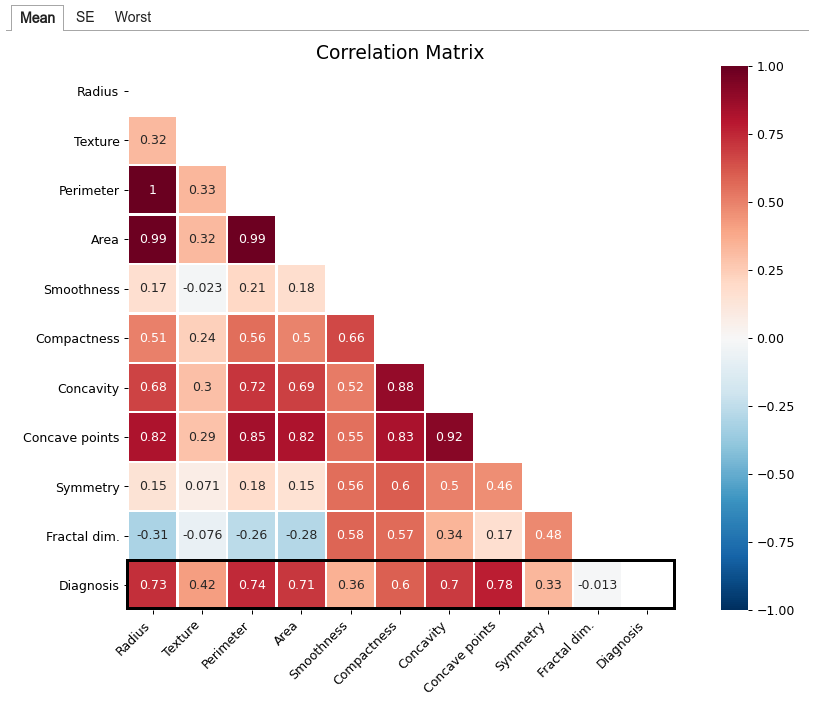
\includegraphics[width=0.935\linewidth, center]{Corr_mean.png}
\end{figure}
$(i) \ \text{\underline{Rows} }  \ 1 : (n-1) : \,$ Based on the linear regression assumptions, independent variables should not be correlated with each other (Multicollinearity). As can be seen, the Radius ($\, r \,$) and the Perimeter ($\, P\, $) have almost $\, 100 \% \,$ correlation score, apparently since most samples are circular and $\,P \propto r \,$. Therefore, one of the features is redundant to another (provide same information) and can be removed to ease calculations and reduce overfitting.

$(ii)  \ \text{\underline{$n$-th Row} } : \,$ Contrarily to $(i)$, here the correlation expresses the feature relevance to the target (\textbf{diagnosis}). Higher values mean higher contribution / relevance. For example, the Radius, Texture, Area, Concavity exhibit ($\geq 70 \% $), while Fractal dimension $(\sim 1 \%)$. 

In order to extract maximum relevance from entire $X$, it can be applied on all 30 features :
\begin{figure}[H]
\centering
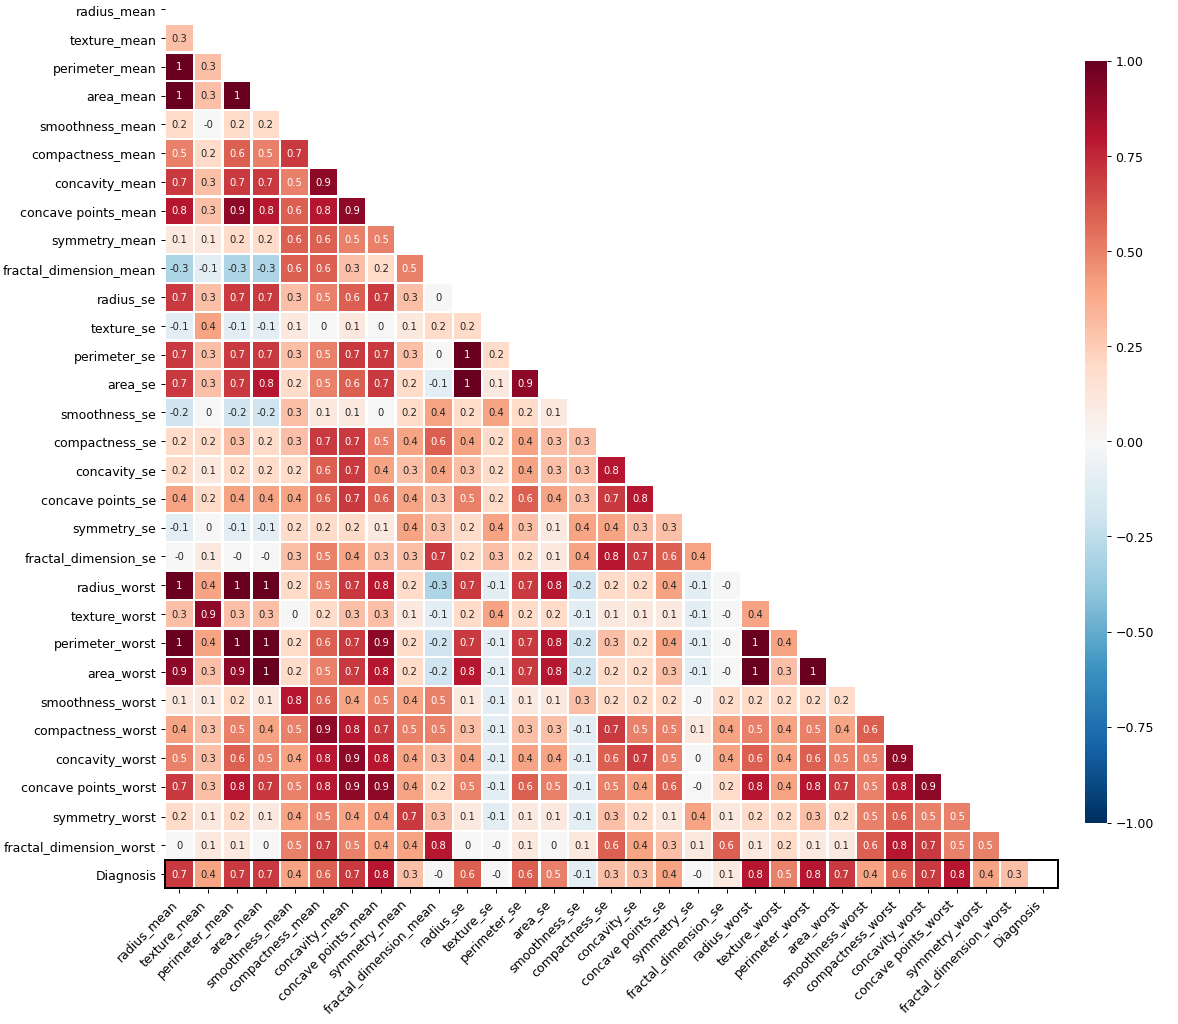
\includegraphics[width=1.115\linewidth, center]{Corr_full_rect.png}
\end{figure}

\section{The Method}
I. \, Extract the most significant features and reduce their dimensionality ($d_0 > d_1 > d_2$) :
\begin{align*}  
X_0 \in \mathbb{R}^{n \times d_0} \quad \underset{\text{Feature selection}}{\Rightarrow} \quad X_1 \in \mathbb{R}^{n \times d_{1}} \quad \underset{\text{Dim. compression}}{\Rightarrow} \quad X_2 \in \mathbb{R}^{n \times d_{2}}
\end{align*}  
II. Compare the classifiers performances and choose the optimal one : $\, f^* : X_2 \rightarrow Y$

\subsection{Feature engineering}
The values in the bottom rectangle (previous figure) denote the correlation strength of features to the \underline{target}. While most featrues exhibit weak connections - $| {corr} | \leq 0.3$, some are strongly related $| {corr} | \approx 0.8$. Therefore the constraint is simple : features should maximize the correlation to the target but minimize correlation with each other. 
 
To that end, a reliable tool is the random forest regressor,  based on GINI importance  [\ref{Method_GINI}]. The method fits a number of classifying decision trees on different subgroups, and calculates each feature importance as the sum over the number of splits (across all tress), proportionally to the number of samples it splits. Here, on the full feature space : 
\begin{figure}[H]
\centering
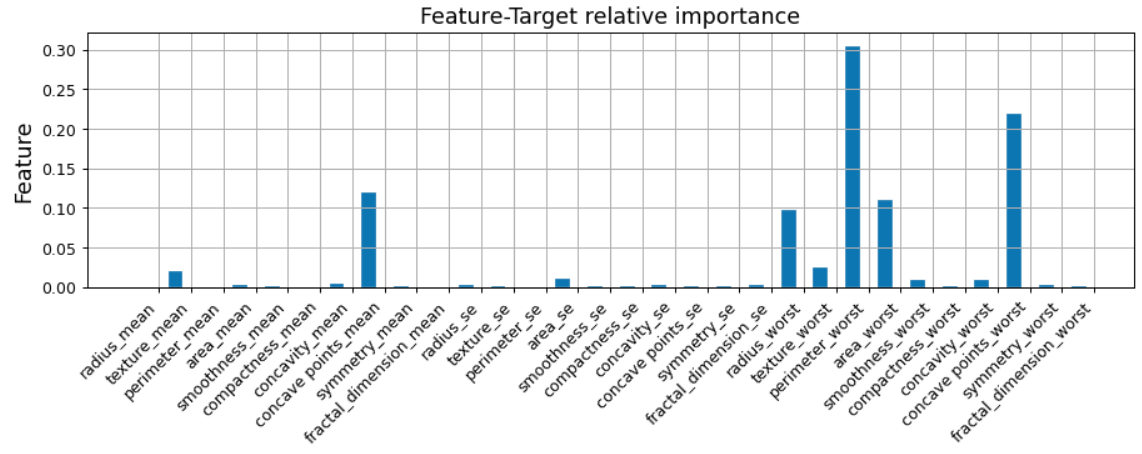
\includegraphics[width=1.075\linewidth, center]{Feature_imp.png}
\end{figure}
As seen before, the Concave points and the perimeter contribute by far more than any other feature. Note that five features manage to contribute up to $80 \%$ of the importance. Using recursive feature elimination (RFE) [\ref{Method_RFECV}], the features are sorted such that high-ranked (informative) features \underline{increase} the model accuracy ($d \leq 16$). But contrastingly, further addition of low-ranked features, would cause a subsequent \underline{decrease} in the accuracy :

\begin{figure}[H]
\centering
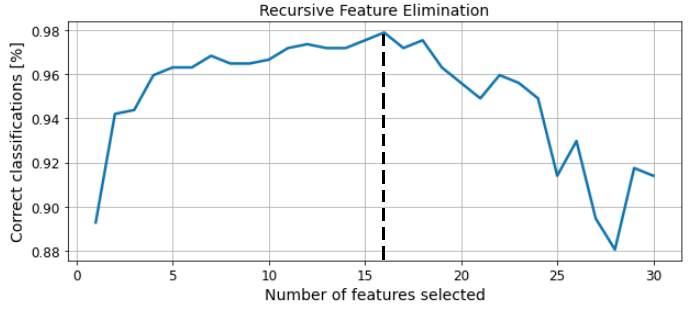
\includegraphics[width=0.9\linewidth, center]{RFECV.png}
\end{figure}

\textbf{Principal component analysis (PCA)} \\[3mm]
PCA is a practical step in dimensionality reduction, by projecting the data from a high-dimensional space onto a lower one. The transformation manages to reveal the internal structure of the data that explains most the data variance (\hyperlink{PCA}{Appendix B}) :
\begin{figure}[H]
\centering
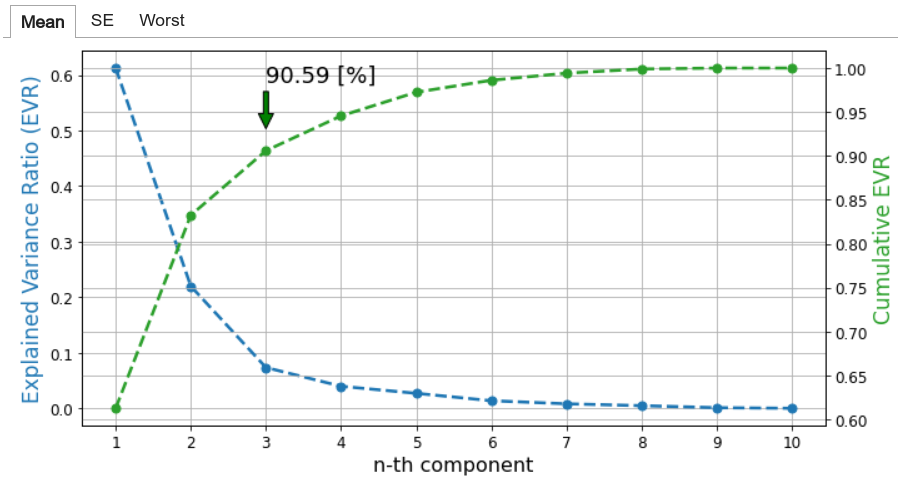
\includegraphics[width=0.95\linewidth, center]{Mat_mean.png}
\end{figure}
The figure above presents PCA on \underline{case (\textbf{a})} ( $X^{(a)}_{\text{Mean}} \in \mathbb{R}^{n \times 10}$ ). From left is the PCA ability to capture proportional variance (EVR), and from right is the cumulative sum.

Let $\, \mathbf{W} \in \mathbb{R}^{10\times10} \, $ be a weights matrix whose columns are the eigenvectors of $X^T X$.  By choosing \textbf{W}'s top 3 eigenvectors, the observations can be projected onto a 3D space :
\begin{figure}[H]
\centering
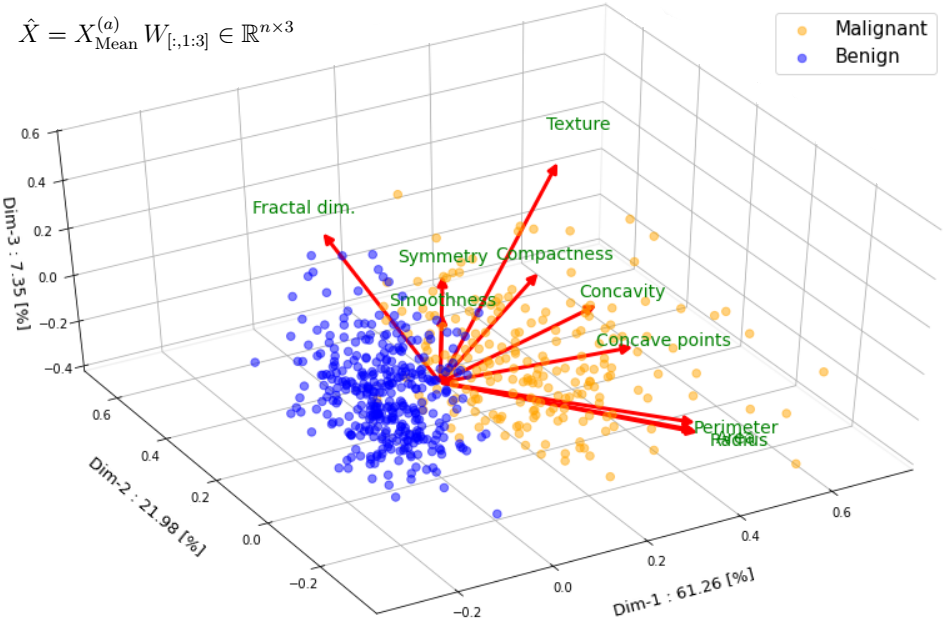
\includegraphics[width=0.935\linewidth, center]{PCA.png}
\end{figure}
Each variable (feature) that went into PCA has an associated red arrow (after scaling factor), in the directions that maximize each of the PC's variance [\ref{PCA}]. Here, the Concave points feature (strong correlation), maximizes the \underline{1st PC}. Contrarily, Fractal dimension and Symmetry, contribute poorly to the \underline{3rd PC}. Therefore, the \underline{full} dataset will undergo :
\begin{align*}
X_0 \in \mathbb{R}^{n \times 30} \quad \underset{\text{Feature selection}}{\Rightarrow} \quad X_1 \in \mathbb{R}^{n \times 16} \quad \underset{\text{Dim. compression}}{\Rightarrow} \quad X_2 \in \mathbb{R}^{n \times 3}
\end{align*}
Such that all that is left to do, is to train a prediction function $\, f : X_2 \rightarrow Y \,$ that will be able to classify the compressed data correctly, in terms of selected metrics.

\subsection{Model selection}
The learning procedure defines a model which associates the correct label for each input sample - $\, y_i = f(x_i) \,$. The performance metric on the output space denotes the cost of wrong labeling, where here, the loss is binary : $ l(\hat{y}, \, y) = \mathbb{I}\{\hat{y} \neq y \}$.

\subsubsection{Metrics}
An evaluation metric is a function that measures a classifier performance, thus allows comparison between models. The confusion matrix from left, defines different combinations for a single indication ( \textbf{T} - True, \textbf{F} - False, \textbf{P} - Positive, \textbf{N} - Negative, \textbf{R} - Rate ) : \\[0.75cm]

\begin{figure}[H]
\centering
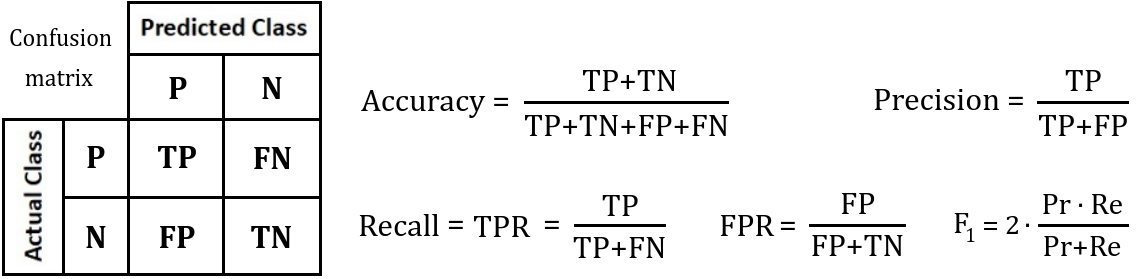
\includegraphics[width=0.95\linewidth, center]{Mat_conf.png}
\end{figure}
Combining the metrics improves understanding of the big picture, and enables to overcome data imbalance. Optimality is obtained by minimizing false indications (\textbf{FP, FN}) : \\[0.75cm]

\begin{figure}[H]
\centering
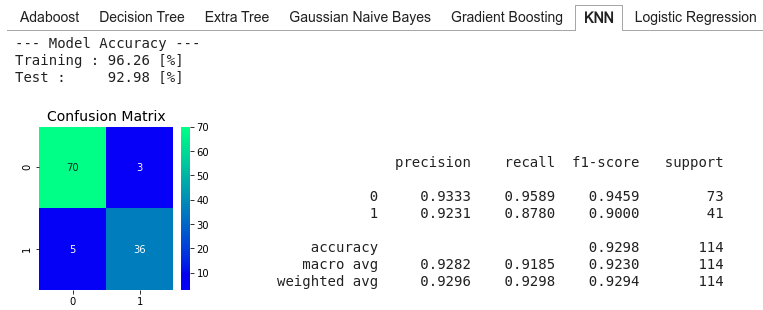
\includegraphics[width=1.05\linewidth, center]{Mat_conf_1.png}
\end{figure}

\textbf{\underline{Note} :} Interactive switching between the tabs is available via the \textit{Colab} version.

\newpage

\subsubsection{Classifiers}
The following list of classifiers was utilized in search of an optimal candidate : \\[5mm]
\begin{tabular}{p{5.5cm} p{5cm} p{5cm}}
\hspace{2cm} $\circ \ $ AdaBoost & $\circ \ $ Gaussian Naive Bayes & $\circ \ $ KNN \\[1ex]
\hspace{2cm} $\circ \ $ Decision Trees & $\circ \ $ Gradient Boosting  &  $\circ \ $ SVM \\[1ex]
\hspace{2cm} $\circ \ $ Extra Trees & $\circ \ $ Logistic Regression & $\circ \ $ Random Forest
\end{tabular}

An \textbf{ROC} reflects a binary classifier ability to discriminate classes, using a probabilistic analysis. Each \underline{threshold} is a point on the \textbf{ROC} graph, denoting the TPR/FPR tradeoff. $\circ \ $ \underline{What would} happen if we took features that scored \underline{poorly} in the correlation matrix ?
\begin{figure}[H]
\centering
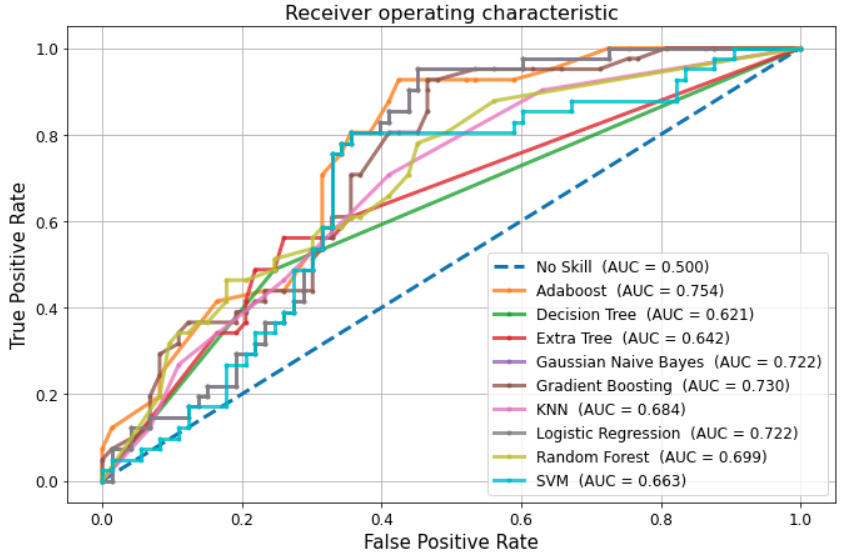
\includegraphics[width=0.825\linewidth, center]{ROC_bad.png}
\end{figure}
Features with low-ranked contribution to the explained variable perform \underline{poorly}, slightly above a random decision / "No skill" (\textbf{AUC}=0.5). The \textbf{AUC} is the area under the \textbf{ROC}, which expresses the prediction success rate from 0-1. Ideally, the perfect classification will exhibit a $ \Gamma$-shape that crosses the (0, 1) point in the FPR-TPR plane. Meaning that there exists a threshold with $100 \%$ correct indications.

Next is the results section, implementing the pipeline on the full dataset :
\begin{align*}
X_0 \in \mathbb{R}^{n \times 30} \quad \underset{\text{Feature selection}}{\Rightarrow} \quad X_1 \in \mathbb{R}^{n \times 16} \quad \underset{\text{Dim. compression}}{\Rightarrow} \quad X_2 \in \mathbb{R}^{n \times 3}
\end{align*}

\section{Results}
Below is a comparative analysis of the chosen classifiers :
\begin{figure}[H]
\centering
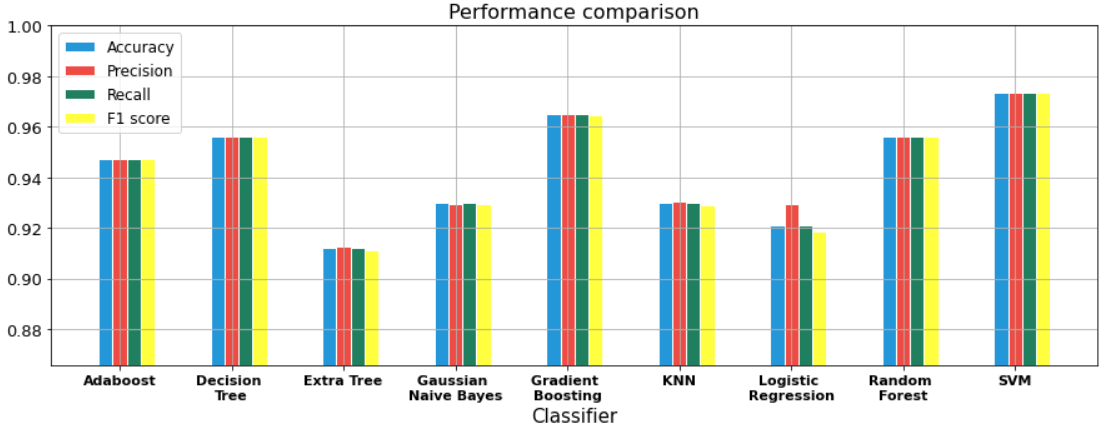
\includegraphics[width=1.125 \linewidth, center]{Results_0.png}
\end{figure}
Similarly, using the FPR/TPR values for calculating the \textbf{AUROC} :
\begin{figure}[H]
\centering
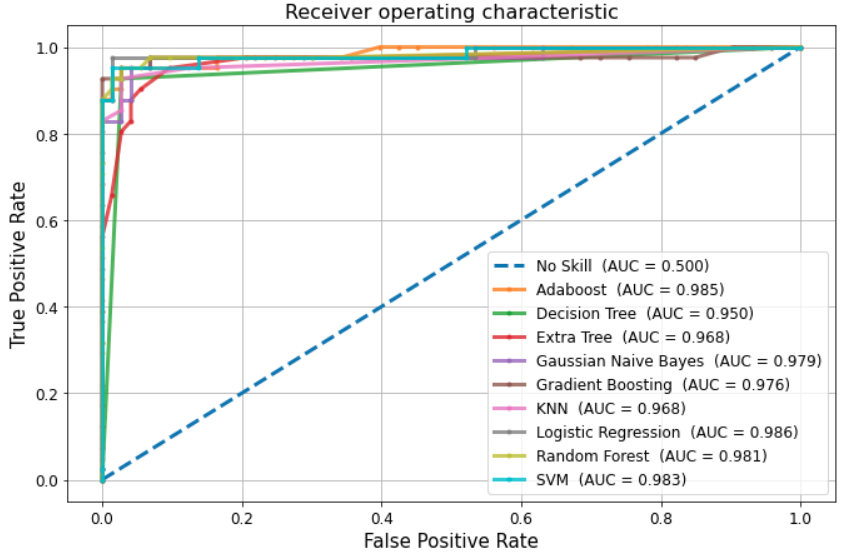
\includegraphics[width=0.885 \linewidth, center]{Results_1.png}
\end{figure}
All of the classifiers succeeded well on the discrimination task. Those who excelled :

\begin{table}
\centering
\begin{tabular}{|c|c|c|c|}
\hline
\textbf{Algorithm} & \textbf{Accuracy} & $F_1$ \textbf{score} & \ \textbf{AUC} \\ \hline
SVM \hspace{2.2cm} & $97.38 \%$ & $97.28 \%$ & $0.9833$  \\ \hline
Gradient Boosting & $96.57 \%$ & $96.51 \%$ & $0.9761$  \\ \hline
Random Forest \hspace{4mm} & $95.66 \%$ & $95.60 \%$ & $0.9811$  \\ \hline
\end{tabular}
\caption*{Top-3 classifiers}
\end{table}

\subsection{Bonus : decision boundary}
Consider an additional PCA, this time to a 2D plane. Using the amazing [\href{http://rasbt.github.io/mlxtend/user_guide/plotting/plot_decision_regions/}{mlxtend}] library, the decision boundary obtained by each one of the classifiers, can be demonstrated as :
\begin{figure}[H]
\centering
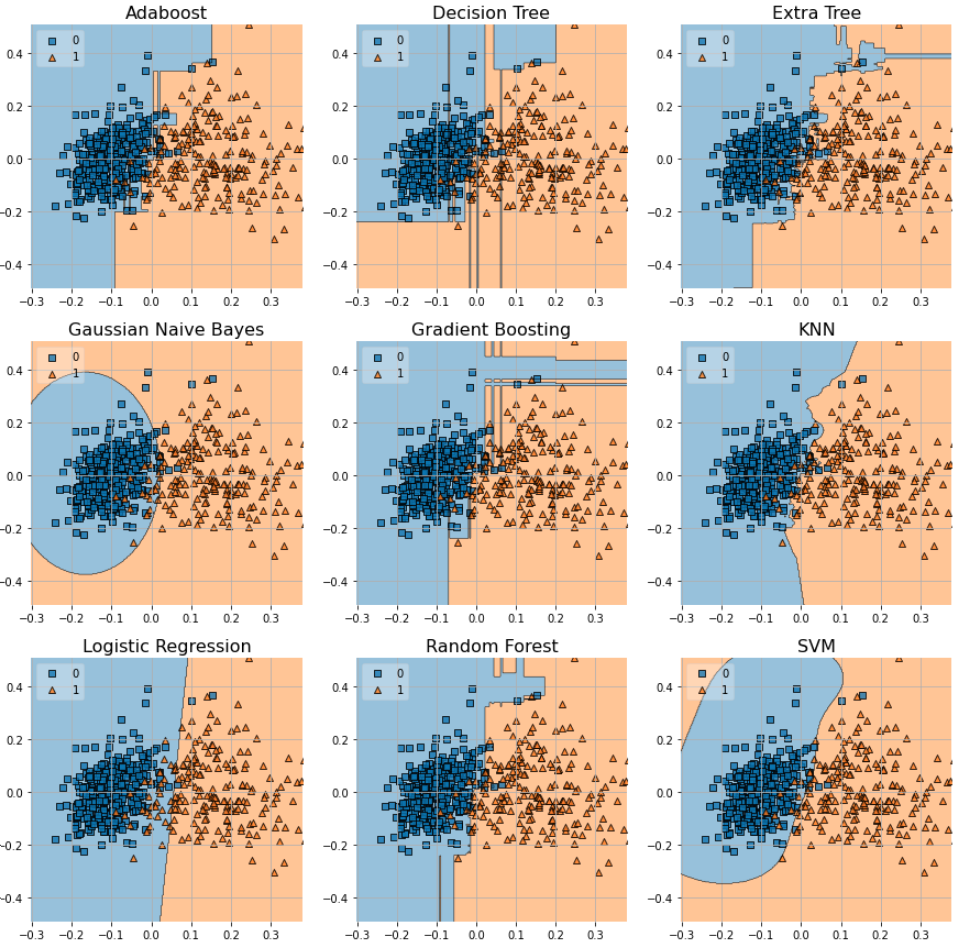
\includegraphics[width=0.985 \linewidth, center]{Decision.png}
\end{figure}




\newpage

\section{Discussion}
In this project I examined the use of several classification techniques for breast cancer diagnosis, after reducing the raw data to a lower representation form. All ML algorithms exhibited high performance on the binary classification, as measured by the chosen metrics.

As a project course, the scope of work is eventually limited to an amount of \underline{15 pages} long. Therefore, hyperparameter optimization and other useful heuristics could not be included.

\subsection{Limitation of the study}

\textbf{Prior engineering} : The dataset as it is publicly available, is already after analysis with specific features, chosen by the researchers. Thereby, the user has no access to the raw image scans at full dimensionality. Thus leaving fewer options for action.


\textbf{Low-dimensional representation} : The process of extraction (by correlation), and then projection (by PCA), ends up with 10 times smaller feature space. Both operations rely on existence of \underline{linear relationships} between the features. This hidden presumption may not always be true, and it might ignore important features that simply fail to score well.

\textbf{Dataset aspect} : The dataset contains a modest amount of samples, distributed at an imbalanced $(B/M)$ ratio of $1.684$. During training, most classifiers reached an accuracy of $100 \%$ (unlike test results), probably due to overfitting. However, rebalance technique that involved up-sampling of the malignant class, did not show any dramatic improvement.

\subsection{Conclusions}

Prediction model for classifying a target variable is statistical by nature. The results range crossed the $90 \%$ accuracy bar. Future work should refer to the limitation of the current project, and can be further challenged by unsupervised learning techniques.

To sum up, I find the project very instructive as I saw by myself how machine learning tools can be implemented wisely in context of healthcare, and yield satisfactory results.

\newpage

% ------------------------------------------------------------------------------ %
\begin{thebibliography}{9} \addcontentsline{toc}{section}{References}
\thispagestyle{empty}

\bibitem{Intro_1} \label{Intro_1}
NCI. January 1980. Archived from the original on 25 June 2014. Retrieved 29 June 2014. \href{https://www.cancer.gov/types/breast}{National Cancer Institute}


\bibitem{Intro_2} \label{Intro_2}
Saunders C, Jassal S (2009). \href{https://oregon.providence.org/forms-and-information/a/ask-an-expert-breast-cancer-growth-rate/#:~:text=With%20most%20breast%20cancers%2C%20each,for%20two%20to%20five%20years.}{Breast cancer } (1. ed.). Oxford: Oxford University Press. p. Chapter 13. ISBN 978-0-19-955869-8. Archived from the original on 25 October 2015.

\bibitem{Intro_3} \label{Intro_3}
McKinney, S. M., Sieniek, M., Godbole,  \& Etemadi, M. (2020). \href{https://www.nature.com/articles/s41586-019-1799-6.epdf?sharing_token=taEAaI9FuO1v2_qjjgBLCNRgN0jAjWel9jnR3ZoTv0M5zwPVx5jT4z_z-YkUZTBTbM27UWphyoF6vHoR667kKgqCi8GNWj2oxgaEK9QGM_IurywsmLuy55SQ7zLhN1w2PP8xyLENTDrX9WSxGhhJyStKcU7vGDuf95dNqUay8vJNKHD0cUHo3S9xHdNCr5bD0uvYtVx23S0ZlTUQ2yrso9HXWCVUi58098rFD6Xl7bkoJt1i9l60yGUzDsjpE7Ro&tracking_referrer=www.bbc.com}{Google DeepMind}. International evaluation of an AI system for breast cancer screening. Nature, 577(7788).

\bibitem{Intro_4} \label{Intro_4}
Nagendran, M., Chen, Y., Lovejoy, C. A., Gordon, A. C. \& Maruthappu, M. (2020). \href{https://www.bmj.com/content/368/bmj.m689}{IBM research group}. Artificial intelligence versus clinicians: systematic review of design, reporting standards, and claims of deep learning studies. bmj, 368. 

\bibitem{Intro_5} \label{Intro_5}
Jeter, R., Josef, C., Shashikumar, S., \& Nemati, S. (2019). \href{https://arxiv.org/abs/1902.03271}{Emory University}. Does the" Artificial Intelligence Clinician" learn optimal treatment strategies for sepsis in intensive care?. arXiv preprint arXiv:1902.03271.


\bibitem{BG_1} \label{BG_1}
Bennett, K. P., \& Mangasarian, O. L. (1992). \href{https://www.tandfonline.com/doi/abs/10.1080/10556789208805504}{Optimization Methods and Softwares} Robust linear programming discrimination of two linearly inseparable sets. Optimization methods and software, 1(1), 23-34.


\bibitem{BG_2} \label{BG_2}
Street, W. N., Wolberg, W. H., \& Mangasarian, O. L. (1993, July). \href{https://www.spiedigitallibrary.org/conference-proceedings-of-spie/1905/0000/Nuclear-feature-extraction-for-breast-tumor-diagnosis/10.1117/12.148698.short?SSO=1}{International Society for Optics and Photonics}. Nuclear feature extraction for breast tumor diagnosis. In Biomedical image processing and biomedical visualization (Vol. 1905, pp. 861-870). 


\bibitem{BG_3} \label{BG_3}
Mangasarian, O. L., Street, W. N., \& Wolberg, W. H. (1995). Breast cancer diagnosis and prognosis via linear programming. \href{https://pubsonline.informs.org/doi/abs/10.1287/opre.43.4.570}{Operations Research}, 43(4), 570-577.


\bibitem{BG_4} \label{BG_4}
Mangasarian, Y. J., \& Wolberg, W. H. (2000). Breast cancer survival and chemotherapy: a support vector machine analysis. Discret Math Probl with Med Appl Work Discret (\href{https://books.google.co.il/books?hl=en&lr=&id=jxOHV22bOekC&oi=fnd&pg=PA1&dq=wisconsin+breast+cancer+dataset&ots=A62LYkr-6U&sig=cXIudG3489I61CJk7Vc2nsSFnvc&redir_esc=y#v=onepage&q=wisconsin%20breast%20cancer%20dataset&f=false}{DIMACS}) December 8–10, 1999, Volume 55 (p. 1).


\bibitem{BG_5} \label{BG_5}
Pantazi, S., Kagolovsky, Y., \& Moehr, J. R. (2002). Cluster analysis of wisconsin breast cancer dataset using self-organizing maps. Studies in health technology and informatics (\href{https://books.google.co.il/books?hl=en&lr=&id=_H2r7pGUNloC&oi=fnd&pg=PA431&dq=wisconsin+breast+cancer+dataset&ots=8ZNuFZYDmy&sig=odOEVgZ8t2L2qlFqlbBpcaN31UI&redir_esc=y#v=onepage&q=wisconsin%20breast%20cancer%20dataset&f=false}{SHTI}), 431-436.


\bibitem{BG_6} \label{BG_6}
Revett, K., Gorunescu, F., Gorunescu, M., El-Darzi, E., \& Ene, M. (2005, November). A breast cancer diagnosis system: a combined approach using rough sets and probabilistic neural networks. In \href{https://ieeexplore.ieee.org/abstract/document/1630149}{EUROCON} 2005-The International Conference on" Computer as a Tool" (Vol. 2, pp. 1124-1127). IEEE.


\bibitem{BG_7} \label{BG_7}
Huang, M. L., Hung, Y. H., \& Chen, W. Y. (2010). Neural network classifier with entropy based feature selection on breast cancer diagnosis. \href{https://www.sciencedirect.com/science/article/abs/pii/S001048250600076X}{Journal of medical systems}.


\bibitem{BG_8} \label{BG_8}
Belciug, S., Salem, A. B., Gorunescu, F., \& Gorunescu, M. (2010). Clustering-based approach for detecting breast cancer recurrence. In 2010 10th International Conference on Intelligent Systems Design and Applications (pp. 533-538). \href{https://ieeexplore.ieee.org/abstract/document/5687211}{IEEE}.


\bibitem{BG_9} \label{BG_9}
Karthik, S., Perumal, R. S., \& Mouli, P. C. (2018). Breast cancer classification using deep neural networks. In Knowledge Computing and Its Applications. \href{https://link.springer.com/chapter/10.1007/978-981-10-6680-1_12}{Springer}.


\bibitem{BG_10} \label{BG_10}
Abdel-Zaher, A. M., \& Eldeib, A. M. (2016). Breast cancer classification using deep belief networks. \href{https://www.sciencedirect.com/science/article/abs/pii/S0957417415007101}{Expert Systems with Applications}, 46, 139-144.


\bibitem{Method_GINI} \label{Method_GINI}
Nembrini, S., König, I. R., \& Wright, M. N. (2018). The revival of the Gini importance? \href{https://academic.oup.com/bioinformatics/article/34/21/3711/4994791}{Bioinformatics}, 34(21), 3711-3718.


\bibitem{Method_RFECV} \label{Method_RFECV}
Lin, X., Yang, F., Zhou, L., Yin, P. \& Xu, G. (2012). A support vector machine-recursive feature elimination feature selection method based on artificial contrast variables and mutual information. \href{https://www.sciencedirect.com/science/article/abs/pii/S1570023212002929
}{Journal of chromatography} B, 910, 149-155.

\bibitem{PCA} \label{PCA}
Holland, S. M. (2008). Principal components analysis (PCA). Department of Geology, University of Georgia, \href{http://strata.uga.edu/software/pdf/pcaTutorial.pdf}{Athens}, GA, 30602-2501.

\thispagestyle{empty}
\subsubsection*{Images sources}

$\circ \quad$ Page 1 : British scientists develop a genetically modified virus. [\href{https://www.dailymail.co.uk/health/article-6405481/British-scientists-develop-genetically-modified-virus-kills-cancer-cells.html}{dailymail.co.uk}]

$\circ \quad$ Page 1 : Differences Between a Malignant and Benign Tumor. [\href{https://www.pinterest.com/pin/622130135997884973/}{pinterest.com}]

$\circ \quad$ Page 2 : Benign and Malignant Breast Lumps. [\href{https://www.verywellhealth.com/understanding-breast-lumps-both-benign-and-cancerous-430415}{verywell health.com}]


\end{thebibliography}
\newpage

\thispagestyle{empty}
\section*{Appendices}
These part contains developments of the methods used along the work. Many of the explanations were taken from Wikipedia as it delivers clear and instructive details.

\subsection*{\hypertarget{corr_mat}{Appendix A} - Correlation matrix} 

A correlation matrix is a table showing correlation coefficients between every two variables. Each cell in the table shows the Pearson correlation coefficient [\href{https://en.wikipedia.org/wiki/Pearson_correlation_coefficient}{ref}] :

$+1 :\ $ perfect \textbf{positive} linear correlation \\
$\hspace{3.5mm} 0 :\ $ \textbf{no} linear correlation \\
$ -1 :\ $ perfect \textbf{negative} linear correlation

$(i) \hspace{2mm} $ \textbf{feature} vs. \textbf{feature} - Every pair of two independent variables :
\begin{align*}  
\text{corr}(X) = \begin{bmatrix}
1 & \frac{\operatorname{E}[(X_1 - \mu_1)(X_2 - \mu_2)]}{\sigma(X_1)\sigma(X_2)} & \cdots & \frac{\operatorname{E}[(X_1 - \mu_1)(X_n - \mu_n)]}{\sigma(X_1)\sigma(X_n)} \\ \\
 \frac{\operatorname{E}[(X_2 - \mu_2)(X_1 - \mu_1)]}{\sigma(X_2)\sigma(X_1)} & 1 & \cdots & \frac{\operatorname{E}[(X_2 - \mu_2)(X_n - \mu_n)]}{\sigma(X_2)\sigma(X_n)} \\ \\
 \vdots & \vdots & \ddots & \vdots \\ \\
 \frac{\operatorname{E}[(X_n - \mu_n)(X_1 - \mu_1)]}{\sigma(X_n)\sigma(X_1)} & \frac{\operatorname{E}[(X_n - \mu_n)(X_2 - \mu_2)]}{\sigma(X_n)\sigma(X_2)} & \cdots & 1
\end{bmatrix}
\end{align*}

Unlike the off-diagonal entries, the principal diagonal denotes the correlation of each random variable with itself $(= 1)$.

$(ii)$ \textbf{feature} vs. \textbf{target} - Every pair of independent variable with respect to the target.
$$ \rho_{X,Y} = \frac{\operatorname{cov}(X,Y)}{\sigma_X \sigma_Y} = \frac{E[(X-\mu_X)(Y-\mu_Y)]}{\sigma_X\sigma_Y} $$
Due to the symmetry, it is suffice to present the lower triangular.

\subsection*{\hypertarget{PCA}{Appendix B} - Principal component analysis}

"PCA is defined as an orthogonal linear transformation that transforms the data to a new coordinate system such that the greatest variance by some scalar projection of the data comes to lie on the first coordinate (called the first principal component), the second greatest variance on the second coordinate, and so on" [\href{https://en.wikipedia.org/wiki/Principal_component_analysis#Covariances}{ref}].

Consider data matrix $X \in \mathbb{R}^{n \times p}$. Its $k$-th component variance can be iteratively maximized, by subtracting the first $k-1$ principal components (PC) from $\hat{X}_k$ :
$$\mathbf{\hat{X}}_{k} = \mathbf{X} - \sum_{s = 1}^{k - 1} \mathbf{X} \mathbf{w}_{(s)} \mathbf{w}_{(s)}^{\rm T} $$
Then finding the weight vector which maximizes the variance of the new data matrix :
$$\mathbf{w}_{(k)} = \underset{\Vert \mathbf{w} \Vert = 1}{\operatorname{arg\,max}} \left\{ \Vert \mathbf{\hat{X}}_{k} \mathbf{w} \Vert^2 \right\} = {\operatorname{\arg\,max}}\, \left\{ \tfrac{\mathbf{w}^T\mathbf{\hat{X}}_{k}^T \mathbf{\hat{X}}_{k} \mathbf{w}}{\mathbf{w}^T \mathbf{w}} \right\}$$
After $k$ iterations, the procedure gives the remaining eigenvectors of $X^T X$ with the maximum values for the quantity in brackets given by their eigenvalues - \textbf{T = XW}. \\
\textbf{W} is a $p$-by-$p$ weights matrix whose columns are the eigenvectors of $X^T X$, and the corresponding eigenvalues are sorted in a descending order. 

\textbf{Note} : PCA can be also obtained by calculating the covariance matrix or by \textbf{SVD}.


\subsection*{\hypertarget{three}{Appendix C} - Code Access}
\thispagestyle{empty}

The project and the code are completely accessible at for anyone who is interested : \begin{center}
\url{https://github.com/Daniboy370/Machine-Learning}
\end{center}

\begin{center}
- $fin$ -
\end{center}



\end{flushleft}
\end{document}